% Copyright 2004 by Till Tantau <tantau@users.sourceforge.net>.
%
% In principle, this file can be redistributed and/or modified under
% the terms of the GNU Public License, version 2.
%
% However, this file is supposed to be a template to be modified
% for your own needs. For this reason, if you use this file as a
% template and not specifically distribute it as part of a another
% package/program, I grant the extra permission to freely copy and
% modify this file as you see fit and even to delete this copyright
% notice. 

\documentclass{beamer}
% Replace the \documentclass declaration above
% with the following two lines to typeset your 
% lecture notes as a handout:
%\documentclass{article}
%\usepackage{beamerarticle}

\usepackage{graphicx}
\usepackage[utf8]{inputenc}
\usepackage{tabto}
 
\graphicspath{ {img/} }


% There are many different themes available for Beamer. A comprehensive
% list with examples is given here:
% http://deic.uab.es/~iblanes/beamer_gallery/index_by_theme.html
% You can uncomment the themes below if you would like to use a different
% one:
%\usetheme{AnnArbor}
%\usetheme{Antibes}
%\usetheme{Bergen}
%\usetheme{Berkeley}
%\usetheme{Berlin}
%\usetheme{Boadilla}
%\usetheme{boxes}
%\usetheme{CambridgeUS}
%\usetheme{Copenhagen}
%\usetheme{Darmstadt}
%\usetheme{default}
%\usetheme{Frankfurt}
%\usetheme{Goettingen}
%\usetheme{Hannover}
%\usetheme{Ilmenau}
%\usetheme{JuanLesPins}
%\usetheme{Luebeck}
%\usetheme{Madrid}
%\usetheme{Malmoe}
%\usetheme{Marburg}
%\usetheme{Montpellier}
%\usetheme{PaloAlto}
%\usetheme{Pittsburgh}
%\usetheme{Rochester}
%\usetheme{Singapore}
%\usetheme{Szeged}
\usetheme{Warsaw}

\title{Programming with Python}

% A subtitle is optional and this may be deleted
\subtitle{Lesson 3: Writing, Reading and Getting Funky with Functions!}

%\author{F.~Author\inst{1} \and S.~Another\inst{2}}
% - Give the names in the same order as the appear in the paper.
% - Use the \inst{?} command only if the authors have different
%   affiliation.

%\institute[Universities of Somewhere and Elsewhere] % (optional, but mostly needed)
%{
%  \inst{1}%
%  Department of Computer Science\\
%  University of Somewhere
%  \and
%  \inst{2}%
%  Department of Theoretical Philosophy\\
%  University of Elsewhere}
% - Use the \inst command only if there are several affiliations.
% - Keep it simple, no one is interested in your street address.

\date{November 15th, 2016}
% - Either use conference name or its abbreviation.
% - Not really informative to the audience, more for people (including
%   yourself) who are reading the slides online

\subject{Python Lessons}
% This is only inserted into the PDF information catalog. Can be left
% out. 

% If you have a file called "university-logo-filename.xxx", where xxx
% is a graphic format that can be processed by latex or pdflatex,
% resp., then you can add a logo as follows:

% \pgfdeclareimage[height=0.5cm]{university-logo}{university-logo-filename}
% \logo{\pgfuseimage{university-logo}}

% Delete this, if you do not want the table of contents to pop up at
% the beginning of each subsection:
%\AtBeginSubsection[]
%{
%  \begin{frame}<beamer>{Outline}
%    \tableofcontents[currentsection,currentsubsection]
%  \end{frame}
%}

% Let's get started
\begin{document}

\begin{frame}
  \titlepage
\end{frame}

%\begin{frame}{Outline}
%  \tableofcontents
%  % You might wish to add the option [pausesections]
%\end{frame}

% Section and subsections will appear in the presentation overview
% and table of contents.
\section{Introduction \& Recap}

\begin{frame}{Last week's goals}
\pause
\begin{itemize}
  \item We have learnt about conditionals
  \pause
  \item We have used conditionals to make our calculator be able to add, subtract, divide or multiply
  \pause
  \item We have used conditionals to handle errors
  \pause
  \item We have learnt about loops and used them to make our program much more usable
  \pause
  \end{itemize}
  
\end{frame}

\section{Files}


\begin{frame}{Messing with files}
Where should we go now with the calculator?

\pause

We are going to work through a log for our calculator!

\end{frame}

\begin{frame}{File input and output}

\pause

In python, the \textit{myFileObj = open()} function will open a file. \pause When you run \textit{open()} you get an object which represents the file.

\pause

Five modes for opening a file: \pause 

\begin{itemize}
  \item \textit{r} \pause \qquad read \pause
  \item \textit{w} \pause \qquad write \pause
  \item \textit{a} \pause \qquad append \pause
  \item \textit{w+} \pause \qquad read \& write \pause
  \item \textit{a+} \pause \qquad read \& append
  
\end{itemize}

\pause

Which mode should we use for a log for our calculator?

\end{frame}

\begin{frame}


The \textit{myFileObj.close()} function will close a file.

\pause

The \textit{myFileObj.write()} function writes to a file.

\pause

The \textit{myFileObj.read()} function reads from a file.

\end{frame}


\begin{frame}{Reading from a file}

\begin{figure}[h]
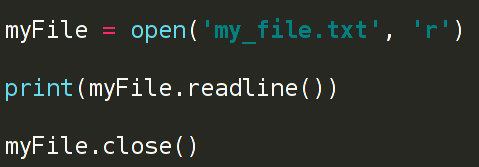
\includegraphics[width=0.8\textwidth]{fileread}
\end{figure}


\end{frame}


\begin{frame}{Writing to a file}

\begin{figure}[h]
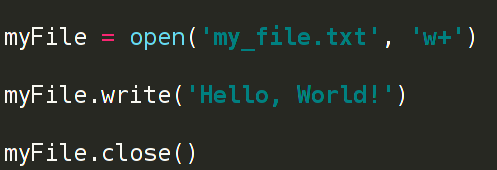
\includegraphics[width=0.8\textwidth]{filewrite}
\end{figure}

\pause

Note, if a file does not exist, it will be created.

\end{frame}

\begin{frame}

Time for a little live coding example!

\end{frame}

\section{Programming Flow}

\begin{frame}{Time for some code cleaning!}

Before we add file IO to our program, we should have a quick look at it.

\end{frame}

\begin{frame}
\begin{figure}[h]
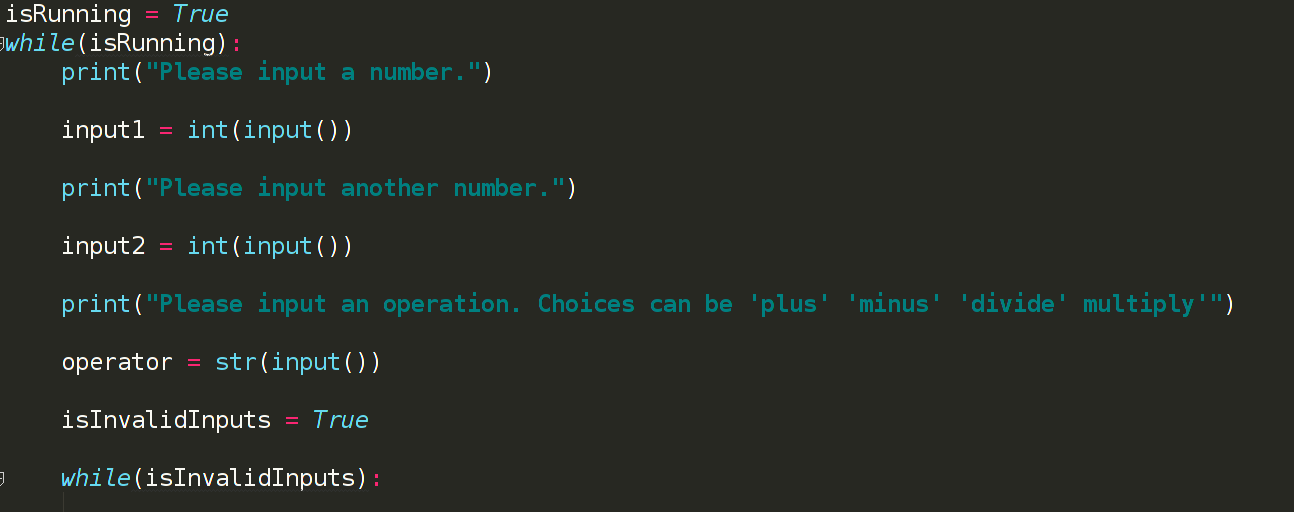
\includegraphics[width=0.99\textwidth]{inputsnip}
\end{figure}
\end{frame}

\begin{frame}
\begin{figure}[h]
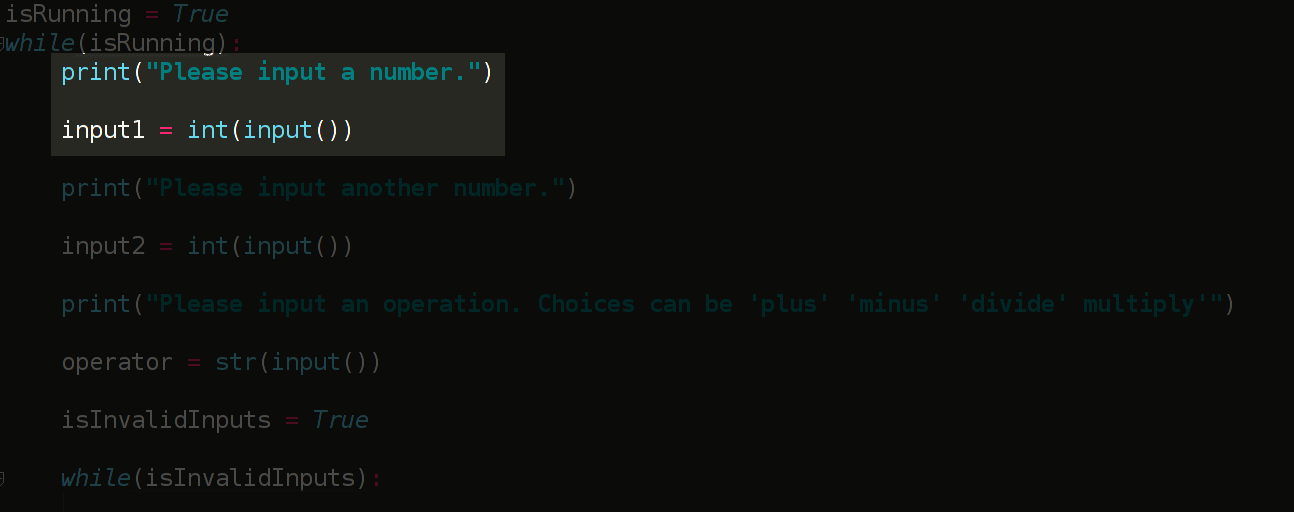
\includegraphics[width=0.99\textwidth]{inputsnip2}
\end{figure}
\end{frame}

\begin{frame}
\begin{figure}[h]
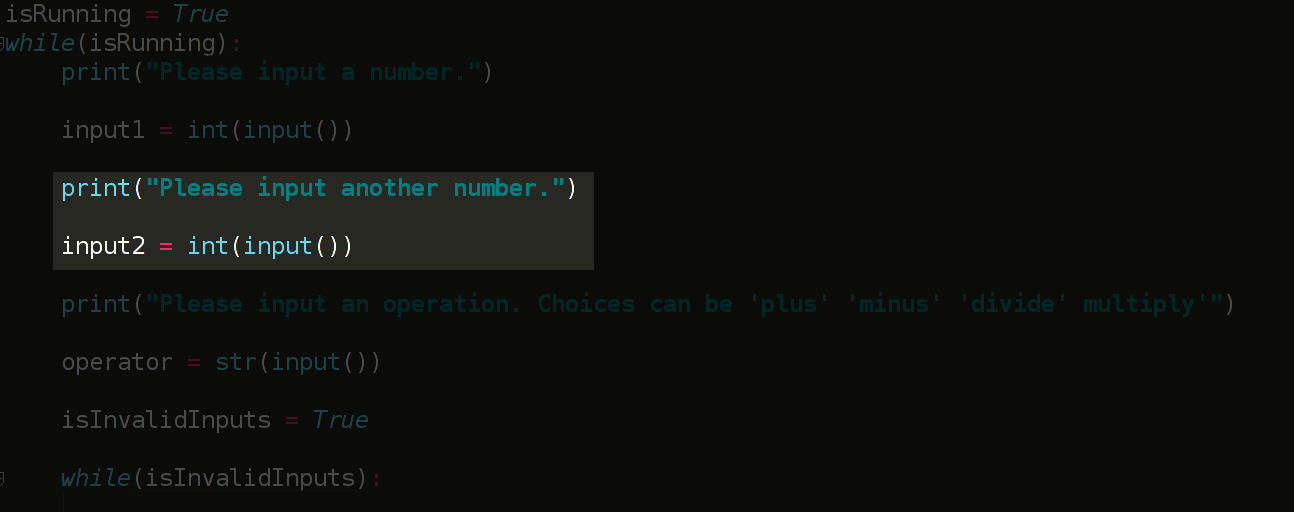
\includegraphics[width=0.99\textwidth]{inputsnip3}
\end{figure}
\end{frame}

\begin{frame}
\begin{figure}[h]
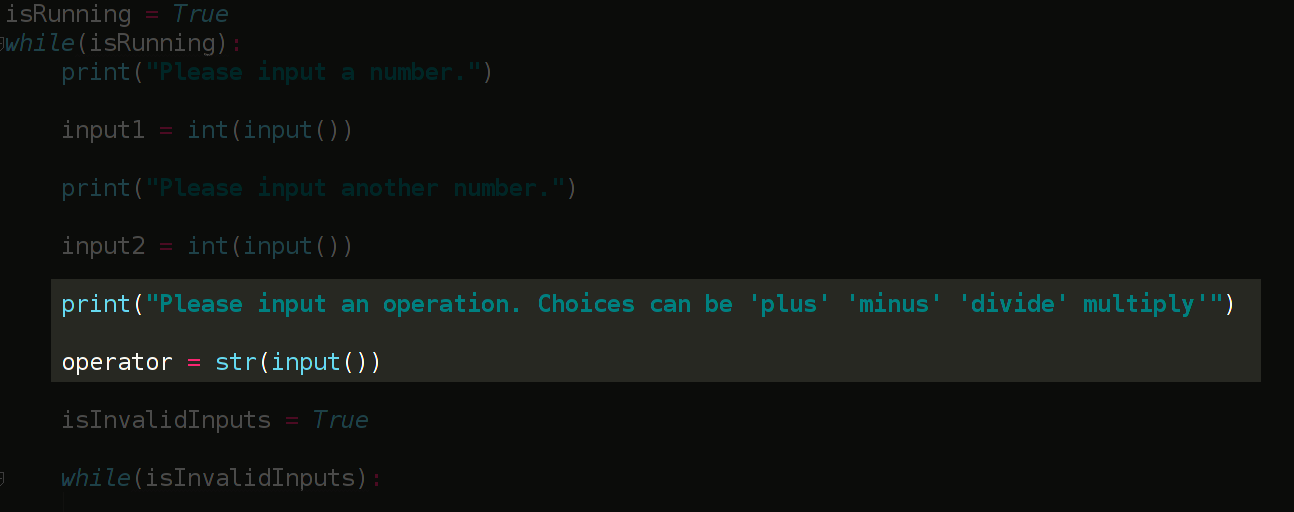
\includegraphics[width=0.99\textwidth]{inputsnip4}
\end{figure}
\end{frame}

\begin{frame}{We don't want to have to repeat ourselves!}

One of the most important rules of good programming is:

\pause

\begin{itemize}

\item[] D \visible<5->{on't}
\item[]\visible<3-> R \visible<6->{epeat}
\item[]\visible<4-> Y \visible<7->{ourself}

\end{itemize}
\visible<8->{
Repeating yourself makes updating/maintaining code horrible and it makes finding bugs in your code impossible!
}
\end{frame}

\section{Functions}

\begin{frame}
\pause
\textbf{Functions} \pause  - the cause of, and solution to all of life's problems!
\end{frame}

\begin{frame}{Getting funky with functions}
\pause
All functions are, are bits of code put together, so we don't have to copy and paste loads of lines everywhere!
\pause
Functions usually take in values (called arguments or parameters) and usually return a value (though this is not always the case).
\end{frame}

\begin{frame}{An example function}

\begin{figure}[h]
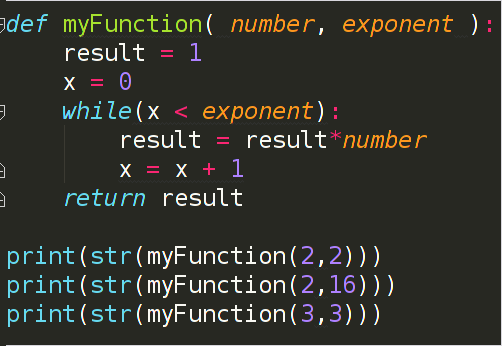
\includegraphics[width=0.7\textwidth]{myfunc}
\end{figure}
\pause
Anyone know what myFunc does?

\end{frame}

\begin{frame}
\begin{figure}[h]
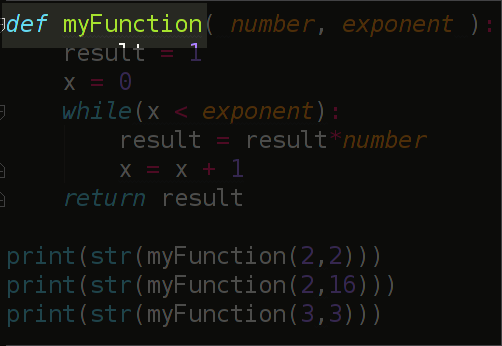
\includegraphics[width=0.8\textwidth]{myfunc2}
\end{figure}
\end{frame}

\begin{frame}
\begin{figure}[h]
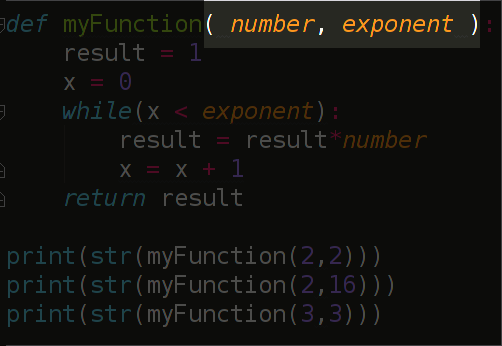
\includegraphics[width=0.8\textwidth]{myfunc3}
\end{figure}
\end{frame}

\begin{frame}
\begin{figure}[h]
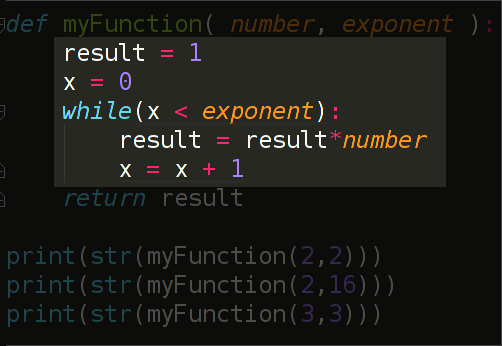
\includegraphics[width=0.8\textwidth]{myfunc4}
\end{figure}
\end{frame}

\begin{frame}
\begin{figure}[h]
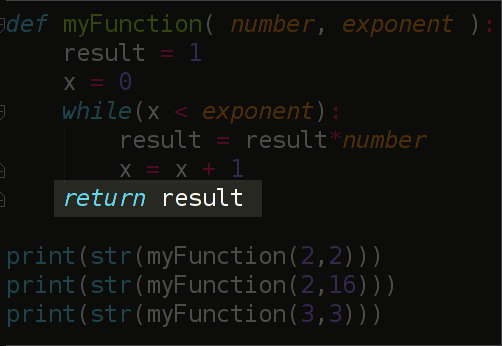
\includegraphics[width=0.8\textwidth]{myfunc5}
\end{figure}
\end{frame}

\begin{frame}
\begin{figure}[h]
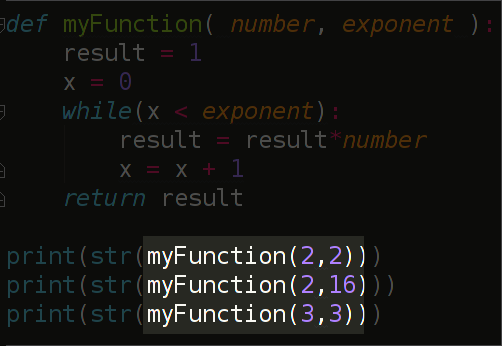
\includegraphics[width=0.8\textwidth]{myfunc6}
\end{figure}
\end{frame}

\begin{frame}{Bringing it all together}

Mega live coding sesh\\
\pause
Challenge: Can anyone make a program which reads out the log?

\end{frame}

\section{Comments}

\begin{frame}{Comments}
Comments are lines in your code which don't do anything.
\pause
They are normally used to help explain the code.
\end{frame}

\begin{frame}
\begin{figure}[h]
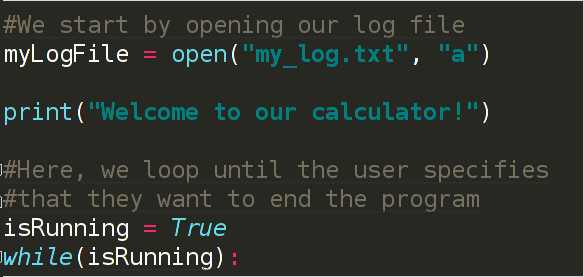
\includegraphics[width=0.8\textwidth]{comment}
\end{figure}
\end{frame}

\section{Summary}

\begin{frame}{That's all for tonight}
  To summarise:
  \pause
  \begin{itemize}
  \item We have learnt about opening and closing files
  \pause
  \item We have learnt to write to, and read from files using the file object
  \pause
  \item We have learnt about the importance of functions and keeping code clean
  \pause
  \item We have used functions to make our code more readable, as well as to write to a log
  \end{itemize}
\end{frame}

\begin{frame}{For next week}
Source code plus lecture slides will be available online soon after the lesson.\\
If you are new to HackSocNotts, please join us on \textit{http://hacksocnotts.slack.com}.\\
If you have any questions, feel free to ask now or over slack.\\
\end{frame}

\end{document}


